\chapter{Étude préalable}

Nous allons exposer tout au long de ce chapitre une synthèse des notions théoriques que nous avons élaboré sur des concepts technologiques qui feront par la suite la base de notre pratique, c'est en effet le contenu de la partie "État de l'art".
À la fin, nous étudions et critiquons des l'existant afin d’introduire notre solution et la positionner par rapport à ce qui existe déjà. \\

\section{État de l'art}
Dans cette section, nous nous intéressons à présenter les deux systèmes utilisés pour la communication des sites aériens; ADAMS et STANOS, tout en définissant leurs compositions et leurs architectures. 
\subsection{Présentation générale du système ADAMS}
\subsubsection{Contexte général}
Le système ADAMS  (Aeronautical Data And Message Handling System) est le système autocommutateur des messages aéronautiques, mis en service en Tunisie depuis l’année 2008  pour l’enregistrement, le traitement et l’acheminement des messages aéronautiques. \\

Il est doté de fonctions et d’outils de contrôle et de supervision permettant d’assurer le bon fonctionnement  des processus de traitement des messages aéronautiques sur le réseau AFTN/AMHS conformément aux recommandations de l’Organisation de l’Aviation Civile Internationale OACI.

\subsubsection{Supervision et exploitation du système}

Le système ADAMS est supervisé 24H par des opérateurs qui assurent le contrôle des différentes opérations et actions se rattachant au système ainsi que la supervision de l’état du réseau d’exploitation sur lequel il opère. Cette supervision continue du système est réalisée  via un système approprié de commandes.\\

Les superviseurs exécuteront leurs tâches quotidiennes sur le système ADAMS à travers les positions MCP (position de contrôle et de supervision des messages et des liaisons) qui sont des stations de supervision connectées directement au central via le réseau LAN, cette tâche consiste à: \\
\begin{itemize}
\item Envoyer et recevoir des messages de formats AFTN ou AMHS.\\
\item Recevoir des messages de format SITA.\\
\item Superviser les différentes activités d’acheminement.\\
\item Vérifier l’état des lignes et circuits.\\
\item Prendre connaissance de l’état opérationnel du centre.\\
\item Suivre les différentes opérations techniques du système.\\
\end{itemize}

\subsubsection{Système de gestion ADAMS}
Le système de gestion ADAMS est un module logistique responsable de la fourniture des outils de gestion de l’interface Homme Machine via laquelle l’opérateur peut inter réagir avec les différentes fonctionnalités du système et de contrôler, superviser et gérer les différents mécanismes logiciels disponibles pour  mener  à bien le processus d’acheminement des, messages aéronautiques, assurer le fonctionnement correct de la partie matérielle du système et garantir la disponibilité optimal du réseau d’exploitation.

\subparagraph{Système de gestion de l’acheminement des messages sous ADAMS:}

Ce module permet au système ADAMS de supporter les différentes technologies de télécommunications avancées par l’OACI telles que l’AFTN et l’AMHS. En effet via ce module de gestion de l’acheminement des messages sous ADAMS, le centre COM principal de Tunis peut être, à la fois, vu comme étant: \\
\begin{itemize}
\item Un centre AFTN. \\
\item Un «Gateway» AMHS / AFTN. \\
\end{itemize}

\subsubsection{Composition d’ADAMS:}
~~\\ 
~~\\
\textbf{- Deux serveurs:} un serveur de secours et un autre opérationnel. On trouve dans chacun, des disques durs de grandes capacités gérés par un système d’exploitation (linux).\\

\textbf{- Deux MSA (Modular Smart Array):} c’est un équipement composé de plusieurs disques sur lesquels est stockée la base de données du système     ADAMS. On  a un MSA fonctionnel et un autre de secours. Chaque MSA contient 5 disques durs (4 fonctionnels et 1 de secours). On peut aussi ajouter des extensions. Au dessus de chaque MSA on trouve un écran digital qui indique l’état de l’ MSA. \\

\textbf{- Deux routeurs:}  routeur est un dispositif situé en un nœud d'un réseau de données qui détermine, pour chaque trame, paquet ou cellule, la route à suivre dans le réseau. \\

\textbf{- Modem:}  Le modem est un dispositif permettent à deux terminaux (console PC) de communiquer à travers une ligne de télécommunication (ligne téléphonique). Les données des terminaux sont transformées par le modem en signaux électriques  de nature acceptable par le réseau de télécommunication, cette transformation est la modulation et démodulation. \\


\textbf{- Switch (A/B):} (AUTOMATIC SWITCHING SYSTEM) c’est un équipement de commutation automatique à large étendue d’applications. Il permet dans notre cas la commutation entre un équipement principal et un équipement de secours assurant ainsi la disponibilité du système. \\


\textbf{- Deux firewalls:} c’est un élément du réseau, qui a pour fonction de faire respecter la politique de sécurité du réseau. Il est généralement installé dans le réseau local de l’entreprise et permet principalement la protection des ressources (serveurs de fichiers, de messagerie, base de données …etc.) des attaques et des accès interdits.\\ 


\subsubsection{Architecture matérielle du système ADAMS}
Le système central ADAMS se compose de:\\ 
\begin{itemize}
\item ne partie serveur autocommutateur de messages AFTN/AMHS  qui contient deux serveurs HP ProLiant DL380 Génération 7 et un système de stockage externe MSA d2000 formant ensemble un système de cluster. Cette partie serveur effectue, lors de la réception d’un message le traitement, l’acheminement et le stockage des messages aéronautiques dans une base de données. \\
\item Une partie réseau qui assure la liaison du cluster avec les différents clients en utilisant les technologies de communications LAN/WAN, Ligne Spécialisée, liaison satellitaire, RTC, FRAME RELAY et RNIS et les protocoles de communications V24 et TCP/IP. \\
\end{itemize}
\begin{figure}[!h]
\begin{center}
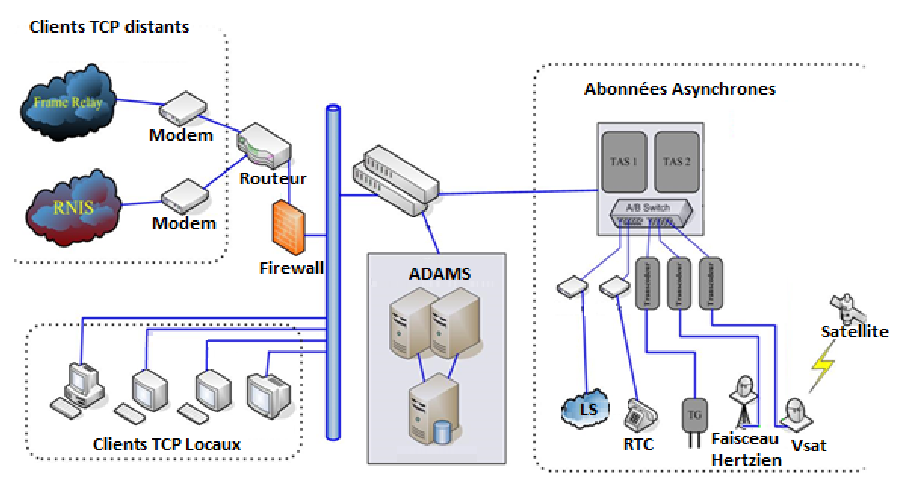
\includegraphics[width=13cm,height=5cm]{existant/architecture.png}
\end{center}
%légende de l'image
\caption{Autocommutateur de message RSFTA}
\end{figure}



\subsection{Présentation générale du système STANOS}
\subsubsection{Contexte général}
A fin d’améliorer sa qualité de service et suivre l’évolution technologique, l’OACA (Office de l’Aviation Civile et des Aéroports) a procédé à l’automatisation du processus d’émission et de réception des messages aéronautiques tels que les \textbf{NOTAM} et \textbf{SNOWTAM}. En effet, l’automatisation de telles tâches peut diminuer le nombre d’erreurs et d’omissions qui peuvent exister au cours de l’exploitation. \\

Par ailleurs, cette tendance d’automatisation des différents processus associés au traitement de l’information aéronautique ne peut être assurée que suite à la création d’une banque de données spécifique de messages aéronautiques regroupant principalement les \textbf{NOTAM} et \textbf{SNOWTAM}. Le logiciel de traitement automatisé des \textbf{NOTAM/SNOWTAM} ou STANOS permet, entre autres, la saisie automatique de ces messages, leur traitement, leur stockage dans la banque de données ainsi que la recherche et la présentation des informations suivant des formats spécifiques tout en satisfaisant un ou plusieurs critères bien déterminés.\\

Le système offre notamment les fonctions suivantes: \\
\begin{itemize}
\item Réception des messages RSFTA (Réseau des Services Fixes des Télécommunications Aéronautiques) à travers les deux liaisons CNA STANOS A et CNA STANOS B reliant le BNI avec le système central d’acheminement des messages aéronautiques ADAMS. \\
\item Validation de tous les NOTAM/SNOWTAM.\\
\item Archivage des NOTAM/SNOWTAM. \\
\item Distribution des NOTAM/SNOWTAM. \\
\item Traitement des messages rejetés. \\
\item Production des bulletins d’information pré-vol PIB en réponse à des requêtes de PIB bien déterminées. \\
\item Diffusion de récapitulatifs de résumés des NOTAM figurant dans la banque de données. \\
\item Création et modification des données géographiques.
\end{itemize}
\subsubsection{Architecture du système STANOS}
\paragraph{Architecture de la base de données STANOS}
~~\\

Le système STANOS est composé d’un ensemble d’applications qui fonctionnent autour d’une base de données distribuée sur plusieurs sites distants. Son fonctionnement est, par conséquent, basé sur une architecture réseau ‘client-serveur’ dont la partie serveur est installée au niveau du Bureau NOTAM International BNI du service de l’Information Aéronautique SIA de la direction de la Navigation Aérienne.\\

La partie serveur comporte des applications spécifiques ainsi qu’une base de données centrale, cette base contient tous les messages aéronautiques NOTAM transmis vers la Tunisie, ces données seront archivés pour des raisons de sécurité de la navigation aérienne (besoins d’enquêtes, traçabilité etc.), tandis que les parties clientes sont installées au niveau des Bureaux d’Information Aéronautique BIA des différents aéroports internationaux tunisiens.\\

Par ailleurs, un module de Distribution sert à alimenter les bases de données locales installées aux niveaux des différents Bureaux d’Information Aéronautique BIA.
~~\\
\begin{figure}[!h]
\begin{center}
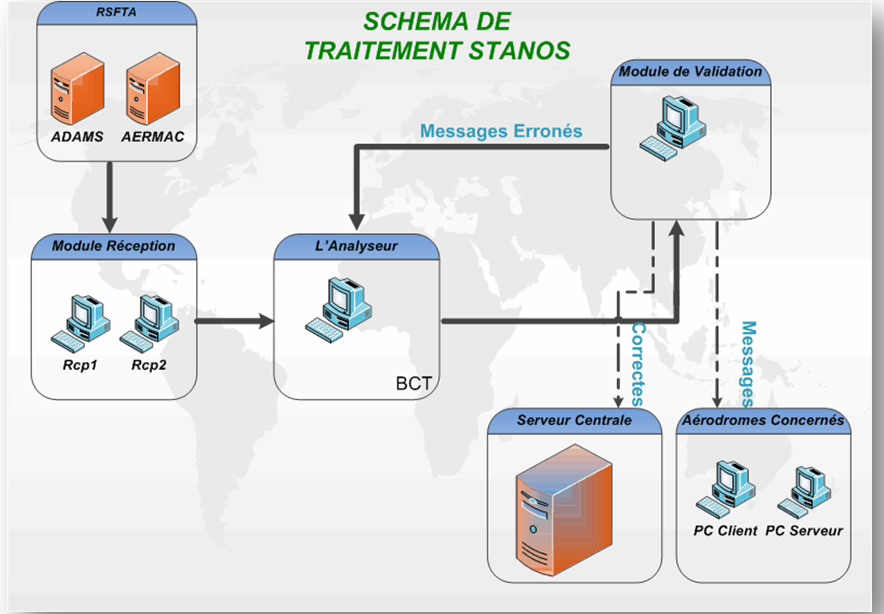
\includegraphics[width=17cm,height=10cm]{existant/architecturestanos.png}
\end{center}
%légende de l'image
\caption{Architecture de la base de données STANOS}
\end{figure}
\newpage
\paragraph{Architecture réseau}
~~\\

Le système STANOS assure la liaison et la distribution des messages aéronautiques NOTAM vers ses clients qui sont les aéroports de la Tunisie: Aéroport International Tunis Carthage, Aéroport International Enfidha Hammamet, Aéroport International Monastir Habib Bourguiba, Aéroport International Djerba Zarzis, Aéroport International Sfax Tina, Aéroport International Tozeur Nefta, Aéroport International Gafsa Ksar, Aéroport International Tabarka Ain Draham.\\

Tous les aéroports sont liés via la liaison Frame Relay sauf l’AITC qui est situé sur le réseau Local du système Central, il est interconnecté via  une liaison fibre optique.   

\begin{figure}[!h]
\begin{center}
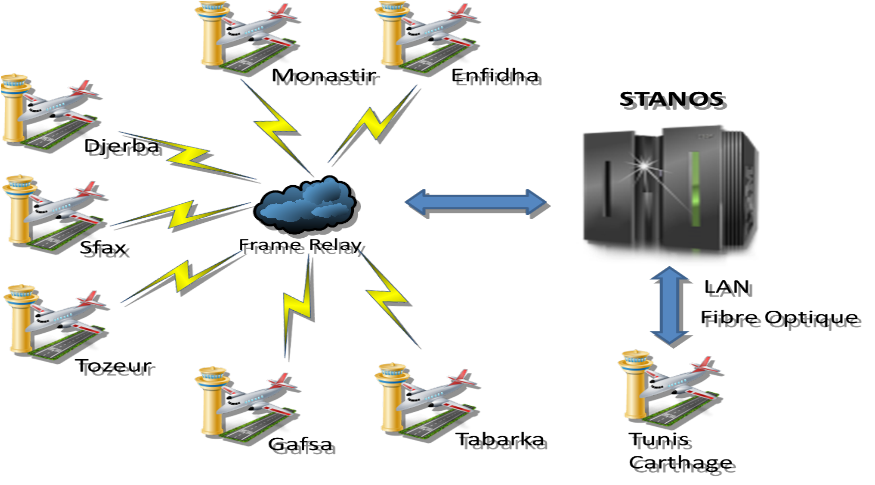
\includegraphics[width=13cm,height=7cm]{existant/stanos.png}
\end{center}
%légende de l'image
\caption{schéma général des liaisons réseaux}
\end{figure}

\begin{figure}[!h]
\begin{center}
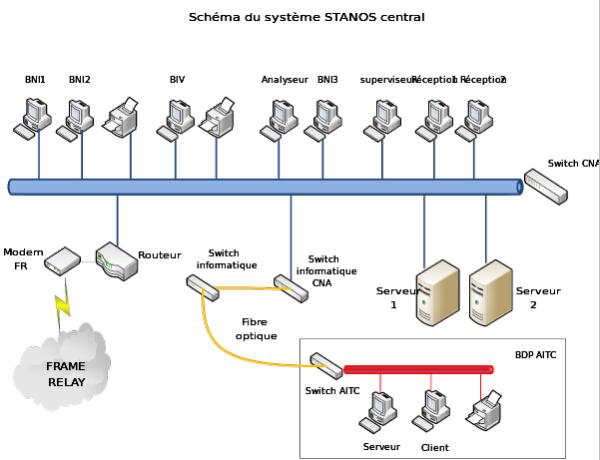
\includegraphics[width=13cm,height=7cm]{existant/Untitled.png}
\end{center}
%légende de l'image
\caption{Architecture centrale du système STANOS}
\end{figure}
\newpage
\paragraph{Fonctionnement global}
~~\\

Dès leur réception sur les lignes RSFTA reliant le Bureau Notam International BNI du service d’Information Aéronautique SIA au système automatique central d’acheminement des messages aéronautiques ADAMS, le système STANOS assure leur traitement immédiat. Ces messages sont ensuite tracés, analysés, validés et enregistrés, au niveau de la base de données centrale du BNI, sous forme d’informations exploitables par les agents d’exploitation de la navigation aérienne  autorisés à cet effet.\\

Le module de distribution ,quant à lui, commence par détecter les nouveaux messages introduits dans la base de données centrale puis analyse sa zone de couverture pour enfin les distribuer vers le ou les Bureaux d’Information Aéronautique concernés au niveau des aéroports internationaux tunisiens. Ainsi, chaque BIA aura une image réduite de la base de données centrale.\\

D’un autre côté, il est à noter qu’au niveau du BIA, l’opération de validation se limite à mettre les messages reçus en zone ou hors zone. Toutes les opérations de traitement (Analyse, correction et validation) se font, de façon centrale, au niveau du BNI.\\


\begin{figure}[!h]
\begin{center}
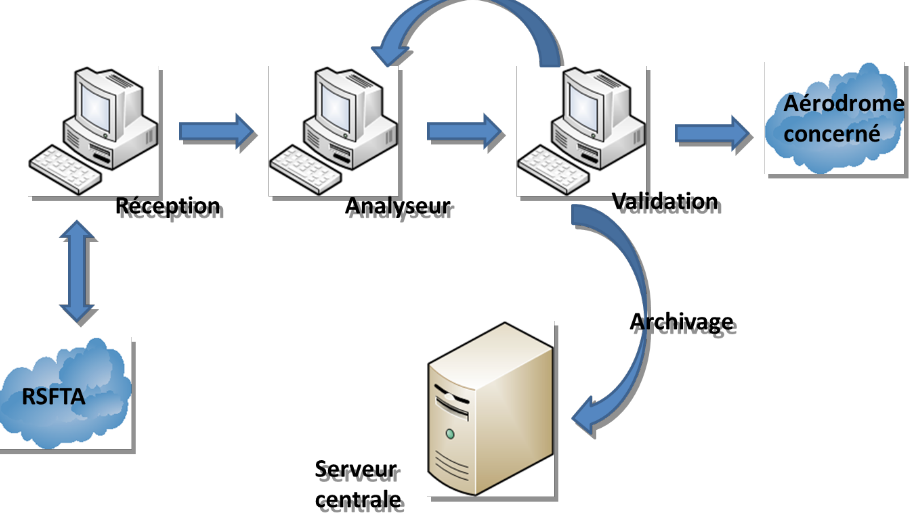
\includegraphics[width=11cm,height=5cm]{existant/fnc.png}
\end{center}
%légende de l'image
\caption{Fonctionnement du système STANOS}
\end{figure}

\section{Etude de l'éxistant}
Le Système autocommutateur de messages aéronautiques assure l’acheminement des messages via deux types de liaisons:\\
\begin{itemize}
\item Liaison synchrone\\
\item Liaison asynchrone\\
\end{itemize}

\subsection{Liaison Synchrône}

Les liaisons synchrones sont utilisées uniquement pour reliés les clients AFTN nationaux.\\
\begin{figure}[!h]
\begin{center}
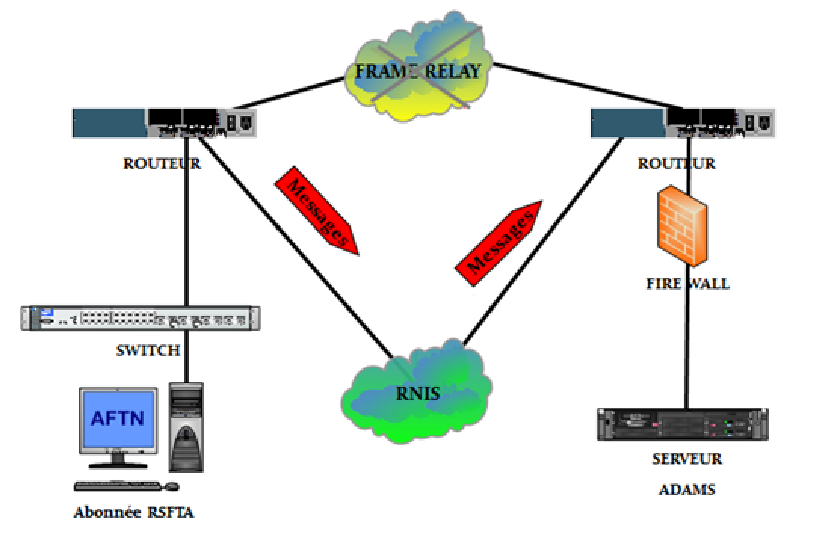
\includegraphics[width=15cm,height=7cm]{existant/sync.png}
\end{center}
%légende de l'image
\caption{Support d’acheminement synchrône}
\end{figure}
 \subsubsection{Frame Relay (Support principal)}
 
 Le Frame Relay est utilisé comme un support de transmission principale pour les échanges entre les différents aéroports. Il établit, en mode connecté, une liaison virtuelle entre les deux extrémités. Cette liaison est permanente (PVC : Permanent Virtual Circuit).\\
 \subsubsection{RNIS (Support de secours)}
 
 Un réseau numérique à intégration de services (RNIS, en anglais ISDN Integrated Services Digital Network) est destiné à remplacer le Frame Relay en cas de panne.\\
Il est caractérisé par :\\
\begin{itemize}
\item Etablissement très court de la communication.\\
\item Débit garanti à 64Kbits/s (et jusqu'à 2Mbits/s).\\
\item Taux d’erreur très faible.\\
\item Cout sur temps de communication.\\
\end{itemize}
\subsection{Liaison asynchrone}

Les liaisons asynchrones sont utilisées  pour acheminer les messages vers les clients nationaux en tant que support de transmission secours en cas de coupure des liaisons synchrones. Seules les abonnées internationales utilisent ces liaisons asynchrones comme des liaisons principales non secourues. \\

\begin{figure}[!h]
\begin{center}
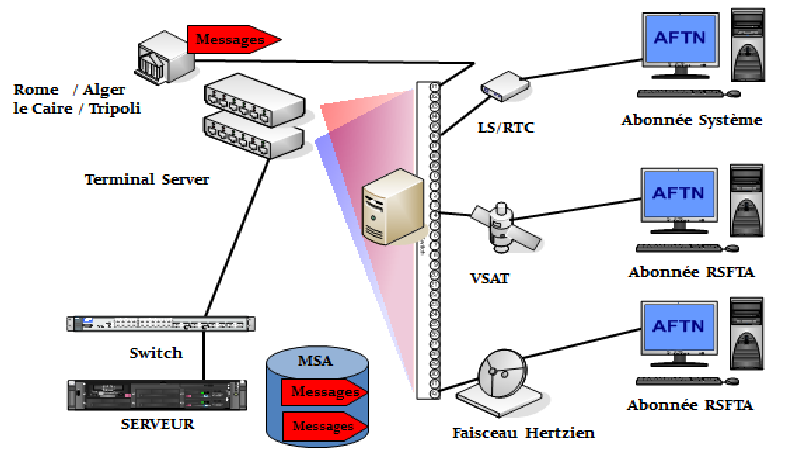
\includegraphics[width=14cm,height=7cm]{existant/asyn.png}
\end{center}
%légende de l'image
\caption{Supports d’acheminement Asynchrone}
\end{figure}
\subsubsection{Faisceau Hertzien}

Le faisceau hertzien est utilisé pour l’acheminement des messages entre le centre de contrôle régional et l’aéroport internationale Habib Bourguiba ainsi que l’aéroport international Enfidha-Hammamet.\\

Un faisceau hertzien est un système de transmission de signaux  entre deux points fixes. Il utilise comme support les ondes radioélectriques, avec des fréquences porteuses de 1 GHz à 40 GHz, très fortement concentrées à l'aide d'antennes directives. Ces ondes sont principalement sensibles aux masquages (relief, végétation, bâtiments…), aux précipitations, aux conditions de réfractivité de l'atmosphère et présentent une sensibilité assez forte aux phénomènes de réflexion\cite{cite4}. \\

\subsubsection{Satellite}

a liaison satellitaire est utilisée pour l’acheminement des messages entre le centre de contrôle régional et l’aéroport international Djerba-Zarzis ainsi que l’aéroport international Sfax-Tina. \\
VSAT est l'abréviation de Very Small Aperture Terminal. Il désigne un terminal terrestre utilisé au sein d'une communication aérienne par satellite pour l'émission/réception de signaux de données. Il s'agit d'une connexion de données haut débit et illimitée.
Un système VSAT consiste en deux parties : une antenne émettrice/réceptrice placée à l'extérieur du centre de contrôle régional pointant vers le satellite de communications, et un dispositif placé à l'intérieur des aéroports distants.\\

\begin{figure}[!h]
\begin{center}
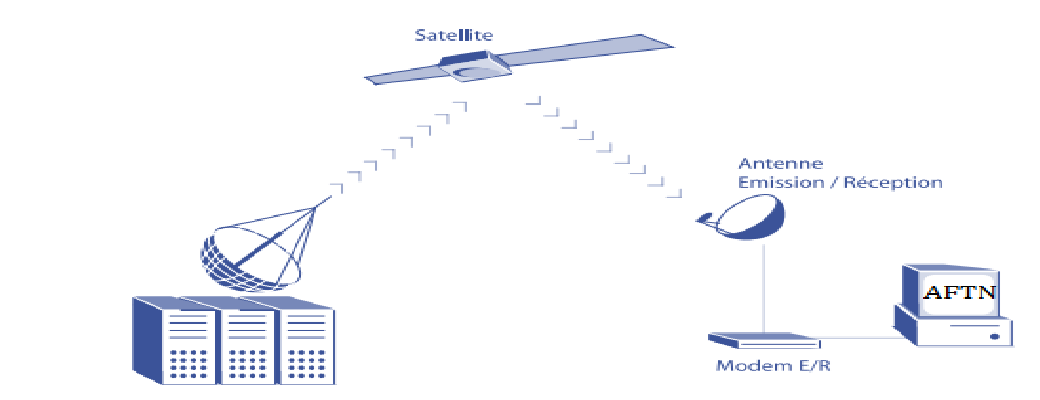
\includegraphics[width=14cm,height=7cm]{existant/sate.png}
\end{center}
%légende de l'image
\caption{Liaison satellitaire}
\end{figure}
~~\\
\subsubsection{RTC (Réseau Téléphonique Commuté)}

La liaison RTC est utilisée pour l’acheminement des messages entre le centre de contrôle régional et l’aéroport international Tabarka-Ain Drahem.\\
Le réseau téléphonique commuté est le réseau du téléphone (fixe et mobile), dans lequel un poste d'abonné est relié à un central téléphonique par une paire de fils. Les centraux sont eux-mêmes reliés entre eux par des liens offrant un débit allant jusqu’à 2 Mb/s Pour établir la communication point à point, l’aéroport AITA et le centre de contrôle régional sont relié à travers deux modems.\\

\subsection{Lignes spécialisées}

Leslignes spécialisées(LS) appelée égalementliaison louée est entélécommunicationune liaison physique de niveau 2, connectée en permanence entre le centre de contrôle régionale de la Tunisie et les autres abonnées internationaux. Elle estmise en œuvreet exploitée par unopérateur de télécommunication sur des longues distances.\\
En réalité la ligne spécialisée n'est souvent dédiée que pour  le site du client et le point d'accès au réseau de l’opérateur de télécommunication.Les données étant transportées ensuite sur des réseaux d'opérateurs de télécommunications, sur lesquels seule la bande passante est dédiée donc elle est onéreuses.\\
\begin{figure}[!h]
\begin{center}
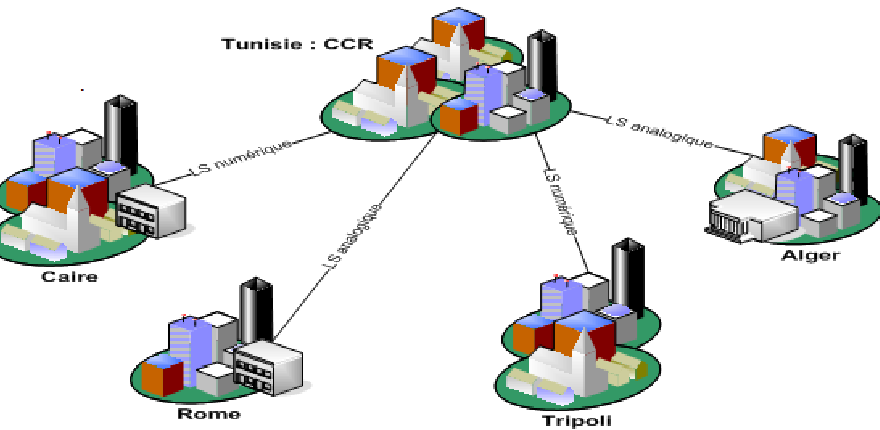
\includegraphics[width=13cm,height=7cm]{existant/ls.png}
\end{center}
%légende de l'image
\caption{Réseau AFTN international}
\end{figure}
\newpage
\subsection{Critique de l'existant}
L’installation du système autocommutateur des messages aéronautiques et du réseau RSFTA/AMHS a bien fonctionné depuis sa mise en marche en 2006. La séparation de traitement des NOTAM des autres messages (les NOTAM sont traités par le STANOS et les autres messages par l’ADAMS) a pour améliorer le temps de réponse et a permis la bonne gestion des messages. Mais après une dizaine d’année d’exploitation, les exploitants de ce système ont remarqué une lenteur importante dans le traitement des messages aéronautiques.  La diagnostique du problème montre que la surcharge du système STANOS par des messages expiré a gravement causé cette lenteur d’où la nécessité d’une opération d’apurement de base de donnée. Pour ne pas tomber dans le même problème prochainement, notre projet de stage consiste à développer une application d’apurement de base de données pour l’utiliser périodiquement dans le but d’assurer le bon fonctionnement de traitement des messages aéronautique.\\
\section*{Conclusion}
Ce chapitre comporte deux sections. La première section intitulée "Etat de l'art" a donné un aperçu sur les deux types de serveurs de messges utilisé au sein de de l'OACA; leurs composition et leurs architectures. La deuxième section a été consacrée à étudier l'exsitant qui nous a aider à révéler leur defaillances et ce afin de déterminer les objectifs et les apports de notre application.
  








%tableau centré à taille variable qui s'ajuste automatiquement suivant la longueur du contenu
% \begin{figure}[!h]
% \begin{center}
% \begin{tabular}{|l|l|l|l|l|}
%   \hline
%   Solution & Critère 1 & Critère 2 & Critère 3 & Critère 4\\
%   \hline
%   Solution 1(cf. ref. \cite{cite0}) & Oui & Oui & Oui & Oui \\
%   Solution 2(cf. ref. \cite{cite1}) & Oui & Oui & Oui & Non \\
%   Solution 3(cf. ref. \cite{cite2}) & Oui (sauf telle chose) & Non & Non & Oui\\
%   Solution 4(cf. ref. \cite{cite3}) & Oui& Non & Oui & Non\\
%   Solution 5(cf. ref. \cite{cite4}) & Oui (uniquement ceux-ci) & Non & Oui & Non\\
%   \hline
% \end{tabular}
% \end{center}
% \caption{Tableau récapitulatif des solutions}
% \end{figure}
